\section{Pruebas}
\subsection{Métricas de rendimiento}
Para evaluar el rendimiento de la implementación y poder comparar ambos protocolos, se han utilizado las siguientes métricas:
\begin{itemize}
    \item \textbf{RTT promedio:} Tiempo entre el envío de un paquete y la recepción de su acuse de recibo.
    \item \textbf{Jitter:} Desviación estándar del RTT.
    \item \textbf{Throughput:} Cantidad de bytes recibidos sobre el tiempo transcurrido.
    \item \textbf{Overhead:} Cantidad de retransmisiones sobre la cantidad de paquetes enviados.
    \item \textbf{Uso promedio de las ventanas de envío y recepción:} Promedio de tamaño de las ventanas de envío y recepción utilizadas durante la transmisión.
\end{itemize}
\subsection{Herramientas utilizadas}
Se utilizó la herramienta \textit{mininet} para simular una LAN simple con tres hosts conectados a través de un switch central. El primer host simula un cliente con una red problemática (10\% de pérdida de paquetes). Los dos primeros hosts están limitados a un ancho de banda de 10 Mbps y a una cola de hasta 1000 paquetes, mientras que el tercer host simula un servidor con una red estable y sin limitaciones de ancho de banda.

Para el cálculo de las métricas mencionadas en la sección anterior, se empleó una estructura de datos que permite almacenar la información necesaria para cada una de ellas. Esta estructura se encuentra en el archivo \texttt{lib/stats/stats\_structs.py} y fue utilizada tanto por el servidor como por los clientes.

\subsection{Escenarios de prueba}
Para evaluar el rendimiento de los protocolos implementados, se generó un conjunto de archivos de prueba con tamaños entre 1 KB y 10 MB. Cada archivo fue transferido utilizando ambos protocolos (Stop \& Wait y Selective Repeat) en distintas condiciones de red simuladas por \textit{mininet} que garantizan una perdida de paquetes del 5 y 10\%.

Cada prueba se repitió cinco veces por archivo, protocolo y condición de red, y se registraron las métricas descritas previamente. Además, las pruebas se llevaron a cabo tanto de forma secuencial como concurrente. En este último caso, se enviaron múltiples archivos de manera simultánea desde diferentes clientes.

\subsection{Resultados obtenidos}

Los resultados obtenidos para los experimentos mencionados se pueden analizar según las siguientes métricas:

\textbf{Tiempo total de transferencia:}
Para la transferencia de archivos pequeños, Stop \& Wait resultó significativamente más rápido que Selective Repeat. Si bien para tamaños más grandes ambos protocolos se equipararon considerablemente, incluso con archivos de 10 MB la diferencia se mantuvo en un rango de 5 segundos.
\begin{figure}[H]
    \centering
    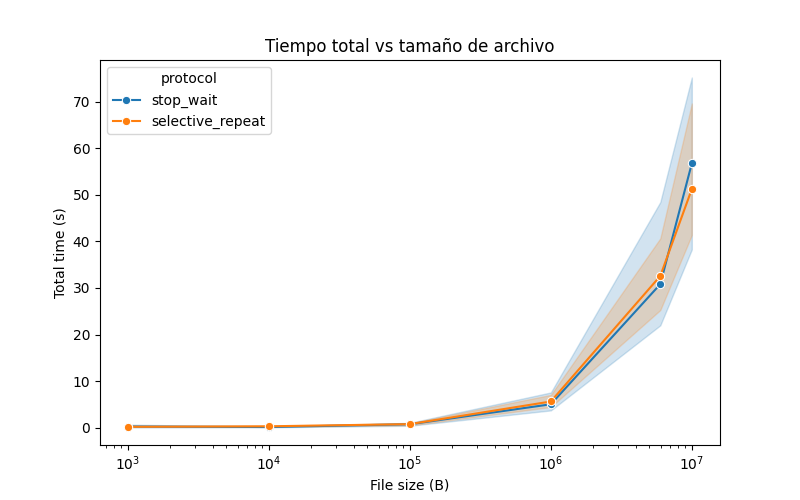
\includegraphics[width=1\linewidth]{images/server_sender_total_time (1).png}
    \caption{Comparación del tiempo total de transferencia entre Stop \& Wait y Selective Repeat}
    \label{fig:total_time_comparison}
\end{figure}

\textbf{Throughput efectivo:}
Consistentemente con la métrica anterior, y probablemente responsable de la misma, el throughput promedio para Selective Repeat fue inferior en la mayoría de los casos. Nuevamente, para archivos más grandes Selective Repeat se acerca e incluso puede llegar a superar a Stop \& Wait, aunque no de manera significativa.
\begin{figure}[H]
    \centering
    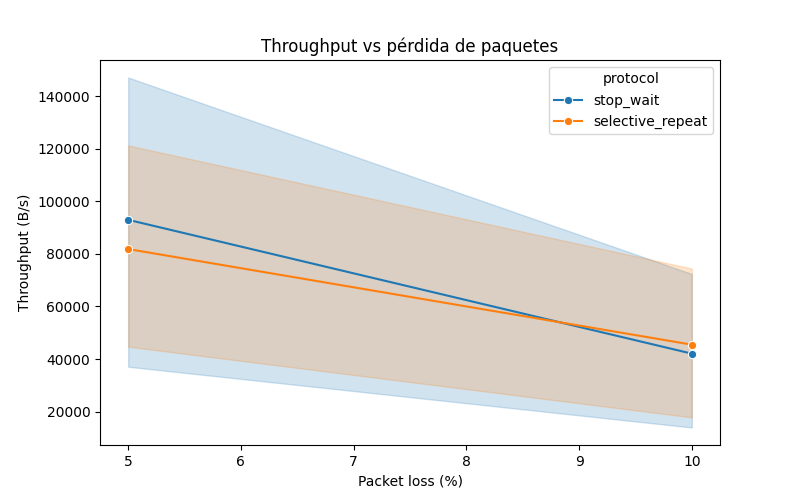
\includegraphics[width=1\linewidth]{images/download_receiver_throughput_loss (1).png}
    \caption{Comparación del throughput efectivo entre Stop \& Wait y Selective Repeat}
    \label{fig:throughput_comparison}
\end{figure}

\textbf{RTT y Jitter:}
Esta fue la métrica más favorable para Stop \& Wait, ya que todos los experimentos realizados con este protocolo obtuvieron menor latencia y mayor estabilidad que Selective Repeat, el cual mostró amplias variaciones entre un RTT y otro.
\begin{figure}[H]
    \centering
    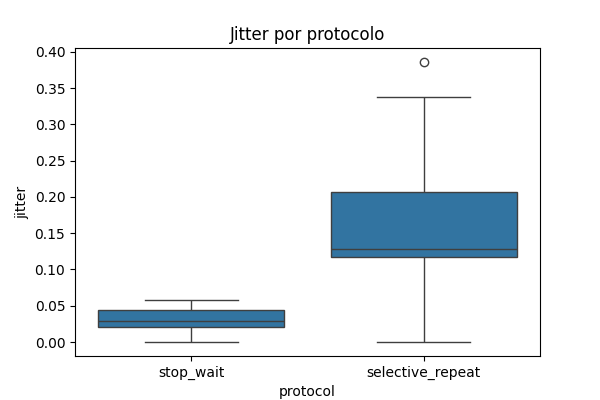
\includegraphics[width=1\linewidth]{images/server_sender_jitter.png}
    \caption{Comparación del Jitter entre Stop \& Wait y Selective Repeat}
    \label{fig:jitter_comparison}
\end{figure}

\textbf{Utilización de la ventana en Selective Repeat:}
Es interesante resaltar este parámetro ya que probablemente sea el responsable del rendimiento inferior de Selective Repeat. Para tamaños de archivos pequeños, el uso no representa ni el 10\% del tamaño total de la ventana, e incluso para archivos de 10 MB el uso alcanza apenas un 50\% de su capacidad total.
\begin{figure}[H]
    \centering
    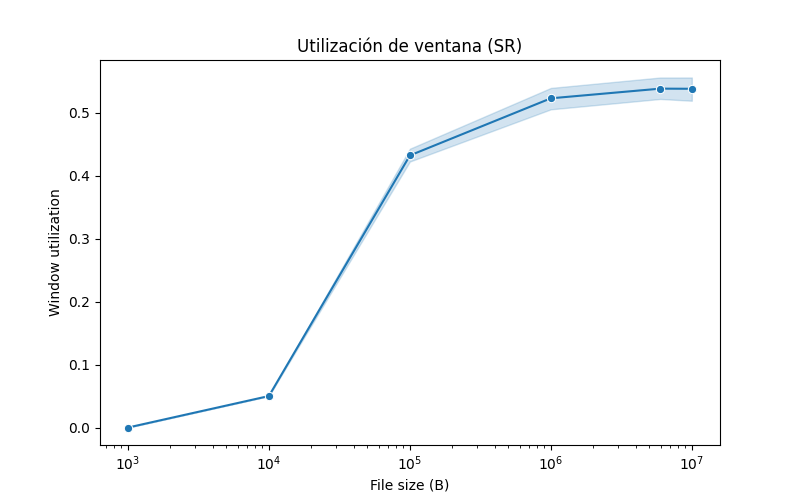
\includegraphics[width=1\linewidth]{images/upload_sender_window_utilization.png}
    \caption{Uso promedio de la ventana de envío en Selective Repeat}
    \label{fig:window_usage}
\end{figure}

El objetivo de estas pruebas era comparar ambos protocolos en condiciones similares. Sin embargo, los resultados obtenidos muestran que Stop \& Wait supera a Selective Repeat en casi todas las métricas evaluadas, incluso en escenarios donde se esperaba que Selective Repeat tuviera un mejor desempeño debido a su capacidad para manejar múltiples paquetes en tránsito. Esto puede atribuirse a varios factores, entre ellos la implementación específica de los protocolos, la configuración de la red simulada y las características inherentes de cada protocolo. Es probable que sea necesario ajustar ciertos parámetros de Selective Repeat, como el tamaño de la ventana o los tiempos de espera, para optimizar su rendimiento en este entorno particular. Además, la sobrecarga adicional que implica la gestión de múltiples paquetes y acuses de recibo en Selective Repeat puede estar afectando negativamente su eficiencia en comparación con la simplicidad de Stop \& Wait. 